% This is samplepaper.tex, a sample chapter demonstrating the
% LLNCS macro package for Springer Computer Science proceedings;
% Version 2.20 of 2017/10/04
%
\documentclass[runningheads]{llncs}
%
\usepackage{graphicx}
\usepackage{latexsym} 
\usepackage{a4wide}
% Used for displaying a sample figure. If possible, figure files should
% be included in EPS format.
%
% If you use the hyperref package, please uncomment the following line
% to display URLs in blue roman font according to Springer's eBook style:
% \renewcommand\UrlFont{\color{blue}\rmfamily}

\begin{document}
%
\title{Runtime Verification For Android Security}
%
%\titlerunning{Abbreviated paper title}
% If the paper title is too long for the running head, you can set
% an abbreviated paper title here
%
\author{Richard Allen \and
Markus Roggenbach\orcidID{0000-0002-3819-2787}}
%
%\authorrunning{F. Author et al.}
% First names are abbreviated in the running head.
% If there are more than two authors, 'et al.' is used.
%


\institute{Swansea University, Swansea, UK\\
\email{ \{998184, M.Roggenbach\}@swansea.ac.uk}
}
%
\maketitle              % typeset the header of the contribution
%
%a) introduce the topic and make it sound interesting.
%
%b) describe the special angle that we take
%
%c) provide technical details of what we do (here, a screenshot would be helpful; also, our monitoring formula for information theft, …)
%
%d) come to a conclusion why the things we have done are important.
%
%See it as a mini-paper reporting on your / our work. 
%
%The 2 pages should be divided roughly as follows:
%
%1/4 page  for a)
%1 paragraph for b)
%1 page for c)
%1 paragraph for d)
%the rest for references

The Android operating system has found many applications in devices
such as phones, tablets, watches and smart TVs. It is characteristic
for these that their primary use is not computation, though they
include a computing system as an integral component. Furthermore,
communication with other external computing systems is essential for
their functionality, i.e., they are open systems by design. As such,
they are vulnerable to typical cyber attacks, including information
theft, service abuse, ransom-ware. Attacks happens to such extent that
the McAfee Q1 2020 threat reports opens with the headline ``Mobile
Malware Is Playing Hide and Steal''.
\footnote{\scriptsize\url{https://www.mcafee.com/content/dam/consumer/en-us/docs/2020-Mobile-Threat-Report.pdf}}

What an app is allowed or is not allowed to do, Android regulates
\emph{statically} with a permission system. However, this system has
known deficiencies. First, apps tend to request for excessive
permissions. Second, users tend to grant permissions to apps without
fully understanding the permissions or their implications in terms of
risk. Third, the permissions system is concerned only with limiting
the actions of individual apps. It is possible for two or more apps to
collude for a malicious action by combining their permissions, even
though each of the colluding apps is properly restricted by
permissions. In a nutshell: under Android, the user does not know what
data an app collects, what an app is doing with that data, or even who
it shares it with: on the device or off the device.

In this context we suggest, similar to \cite{bauer2012runtime} {\bf
  anything to say what we do different?}, to \emph{dynamically}
monitor operating system calls on the device with techniques from
runtime verification in order to alert the user of an Android device
if there is a potential security breach. This will allow the user to
react, e.g., by closing or removing the involved apps. Our approach
comes with a number of advantages:
\begin{itemize}
\item The user is informed immediately when the device is under
  attack.
\item It is independent of the application code.  % put (xposed module automatically generated at run time) in the architecture picture
\item It is extendible to further security properties.
\end{itemize}

In order to illustrate our approach, we use a simple form of
information theft through app collusion as our running example
\cite{collusion17}: two apps $A$ and $B$ combine their permissions in
order to steal some information. To this end, app $A$ first reads the
information, then shares is via Android inter app communication with
app $B$, which finally sends the information off the device. A typical
example for $A$ could be a contact managing app with read and write
access for contacts, however, no Internet access; $B$ could be a
weather app, without access to contacts, however, access to the
Internet in order to obtain the weather forecast. There is evidence of
collusion based cyber attacks in the wild
\cite{PrologAppCollusion}. 

Android apps run in a `sandbox'. Any access to a system resource
requires a call to the operation system. Thus, \emph{conceptually},
information theft through app collusion can be detected by monitoring
operation system calls. For information theft through app collusion to
possibly happen, the following sequence of calls is necessary: app $A$
makes a query $q$ to some resource protected by Android and then
initiates an interapp communication on the device by a send call $s$;
app $B$ makes a receive call $r$ and performs a publish call
$p$. \footnote{Note that a sequence $\langle q, s, r, p \rangle$ of
  operation system calls describes information theft only, if the
  published data can be `traced back' to the queried data.} It it
possible to express such trace properties in linear temporal logic
(LTL). For instance, the LTL formula
%
$$       (\Box s \land (\neg s\ U\ \Box q))
   \land (\Box r \land (\neg r\ U\ \Box s)) 
   \land (\Box p \land (\neg p\ U\ \Box r)) 
$$ 
%
is true if a trace includes the call pattern necessary for information
theft through app collusion.
%
It is possible to express other relevant security properties in LTL,
``alert whenever an app takes an image from the camera'' or ``the
microphone is never activated before a telephone call has been
initiated or accepted''.

In the \emph{technical realisation} of our approach, our system
architecture makes use of the Xposed framework \cite{rovo89} {\bf add
  reference} in order to intercept calls to security sensitive Android
O/S functions. It adds a monitor app to the user's device which logs
these calls and, at arrival of a new event, checks for each security
property of interest if it is fulfilled or not.

\begin{center}
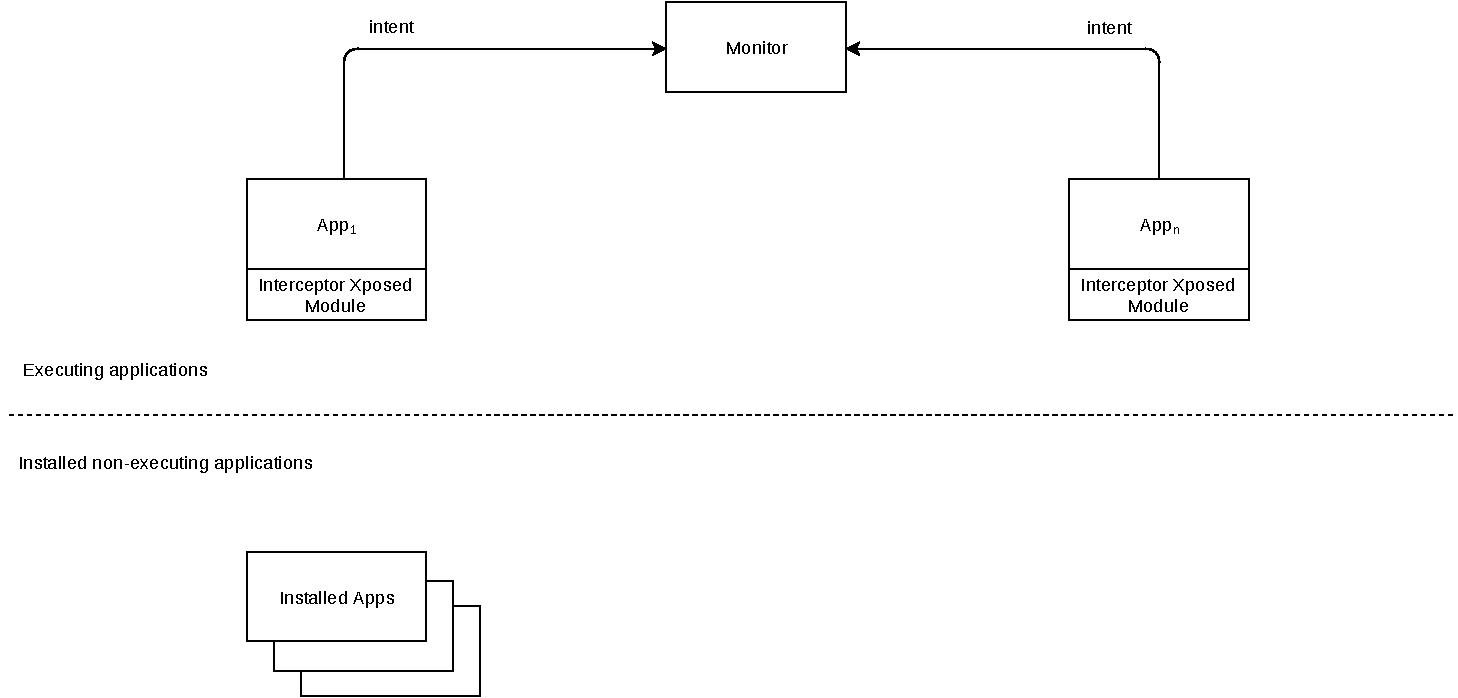
\includegraphics[width=0.7\textwidth]{HighLevelArchitecture.pdf}
\end{center}

In a first attempt to implement the monitor app, we utilised an
algorithm by Rosu and Havelund \cite{RosuHavelund} which appeared to
be interesting thanks to its low complexity: the cost for evaluating a
property $\varphi$ on a trace $t$ is $O(|t| * |\varphi|),$ i.e., is
linear. However, as this algorithm traverses the trace $t$ from the
last event to the first event, it is impossible to re-use intermediate
results from evaluating $\varphi$ on $t$ for evaluating $\varphi$ on
$t {\mathbin{\raise 0.8ex\hbox{$\frown$}}} \langle e \rangle,$ i.e.,
the trace $t$ extended by an event $e.$ In our experiments this limits
the trace length to about 60 events, beyond that, the device did not
respond any more. Such length is far too short to be of any use in a
real world scenario. Thus, we implemented a `reverse' version of this
algorithm that allows for re-use. While our new algorithm performs
well, i.e., traces can grow to arbitrary size (we have tested the
algorithm up to a trace length of {\bf add a number}) without
encountering any issues) and evaluation time for new events is in the
area of milliseconds for the formula stated above, this comes at a
price: our new algorithm does not support the LTL next operator.

By utilising colluding apps developed for testing purposes,
cf.\ \cite{collusion17}, we have successfully demonstrated that our
monitoring approach effectively works on Android hardware and does not
cause any significant performance reductions (occurrence of an event
causes CPU usage in the area of {\bf 1.5\%}). However, further
experimentation, in particular with monitoring simultaneously for
different security properties, will be necessary to completely
evaluate the performance properties of our approach. First experiments
suggest a linear increase in CPU usage with the number of formulae
monitored for.

%[TODO Add some reference to related papers]

\bibliographystyle{abbrv}
\bibliography{doc}

\end{document}
